%% LyX 2.0.0 created this file.  For more info, see http://www.lyx.org/.
%% Do not edit unless you really know what you are doing.
\documentclass[english]{beamer}
\usepackage{mathpazo}
\renewcommand{\sfdefault}{lmss}
\usepackage[T1]{fontenc}
\usepackage[latin9]{inputenc}
\usepackage{color}
\usepackage{amsmath}
\usepackage{amssymb}

\makeatletter
%%%%%%%%%%%%%%%%%%%%%%%%%%%%%% Textclass specific LaTeX commands.
 % this default might be overridden by plain title style
 \newcommand\makebeamertitle{\frame{\maketitle}}%
 \AtBeginDocument{
   \let\origtableofcontents=\tableofcontents
   \def\tableofcontents{\@ifnextchar[{\origtableofcontents}{\gobbletableofcontents}}
   \def\gobbletableofcontents#1{\origtableofcontents}
 }
 \long\def\lyxframe#1{\@lyxframe#1\@lyxframestop}%
 \def\@lyxframe{\@ifnextchar<{\@@lyxframe}{\@@lyxframe<*>}}%
 \def\@@lyxframe<#1>{\@ifnextchar[{\@@@lyxframe<#1>}{\@@@lyxframe<#1>[]}}
 \def\@@@lyxframe<#1>[{\@ifnextchar<{\@@@@@lyxframe<#1>[}{\@@@@lyxframe<#1>[<*>][}}
 \def\@@@@@lyxframe<#1>[#2]{\@ifnextchar[{\@@@@lyxframe<#1>[#2]}{\@@@@lyxframe<#1>[#2][]}}
 \long\def\@@@@lyxframe<#1>[#2][#3]#4\@lyxframestop#5\lyxframeend{%
   \frame<#1>[#2][#3]{\frametitle{#4}#5}}
 \newenvironment{topcolumns}{\begin{columns}[t]}{\end{columns}}
 \def\lyxframeend{} % In case there is a superfluous frame end

%%%%%%%%%%%%%%%%%%%%%%%%%%%%%% User specified LaTeX commands.
\usetheme{Darmstadt}
%\usetheme{Frankfurt}
% or ...

\setbeamercovered{transparent}

\makeatother

\usepackage{babel}
\begin{document}


\title[Short Paper Title]{Singular Value Decomposition}


\subtitle{Why and How}


\author[Author]{Royi Avital}


\date[2011]{June, 2011}

\makebeamertitle


%\pgfdeclareimage[height=0.5cm]{institution-logo}{institution-logo-filename}

%\logo{\pgfuseimage{institution-logo}}



\AtBeginSubsection[]{

  \frame<beamer>{ 

    %\frametitle{Outline}   

    \tableofcontents[currentsection,currentsubsection] 

  }

}



%\beamerdefaultoverlayspecification{<+->}


\lyxframeend{}\lyxframe{}

\tableofcontents{}




\lyxframeend{}\section{Definitions and Notations}


\lyxframeend{}\subsection[Notations]{Notations}


\framesubtitle{}


\lyxframeend{}\lyxframe{}
%\frametitle{Notations}
\begin{itemize}

\item Capital letter stands for a Matrix
$$ A \in {\mathbb{C}}^{mxn}, \ A \in {\mathbb{R}}^{mxn} $$

\item Small letter stands for a column Vector
$$ a \in {\mathbb{C}}^{mx1}, \ a \in {\mathbb{R}}^{mx1} $$

\item Referring a Row of a Matrix
$$ {A}_{i} \ - \ The \ i-th \ Row \ of \ a \ Matrix $$

\item Referring a Column of a Matrix
$$ {A}^{j} \ - \ The \ j-th \ Column \ of \ a \ Matrix $$


\end{itemize}

\lyxframeend{}\subsection[Definitions]{Definitions}


\framesubtitle{}


\lyxframeend{}\lyxframe{}
%\frametitle{Definitions}
\begin{itemize}
\item Unless written otherwise, The Complex Field is the default

\item Conjugate Operator
$$ {A}^{*} $$

\item Transpose Operator
$$ {A}^{T}: {{A}^{T}}_{ij} = {A}_{ji} $$

\item Complex Conjugate Transpose Operator
$$ {A}^{H}:  {{A}^{H}}_{ij} = {{A}_{ji}}^{*} $$

\item Range Space and Null Space of Operator \\
Let $ L: X \rightarrow Y $ be an Operator (Linear or otherwise). The Range Space $ \mathcal{R} \left( L \right) \subseteq Y $ is
$$ \mathcal{R} \left( L \right) = \lbrace y = Lx : x \in X \rbrace $$
The Null Space $ \mathcal{N} \left( L \right) \subseteq X $ is
$$ \mathcal{N} \left( L \right) = \lbrace x \in X : Lx = 0 \rbrace $$


\end{itemize}


\lyxframeend{}\subsection{Introduction}

\lyxframeend{}\lyxframe{}
\begin{itemize}
\item Each Linear Operator $ A : {\mathbb{C}}^{n} \rightarrow {\mathbb{C}}^{m} $ defines spaces as follows \\
\begin{center}
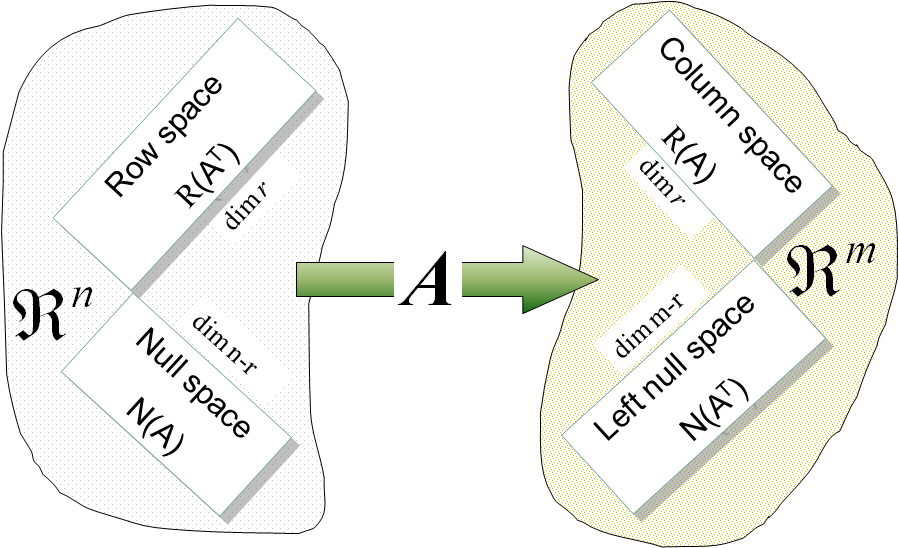
\includegraphics[scale = 0.25]{OperatorSpaces.PNG} 
\end{center}

\item The following properties hold
$$ \mathcal{R} \left( A \right) \bot \mathcal{N} \left({A}^{H} \right), \ \mathcal{R} \left( {A}^{H} \right) \bot \mathcal{N} \left(A \right) $$

$$ rank \left( A \right) = dim \left( \mathcal{R} \left( A \right) \right) = dim \left( \mathcal{R} \left( {A}^{H} \right) \right) = rank \left( {A}^{H} \right) $$

\end{itemize}


\lyxframeend{}\lyxframe{}
\begin{itemize}
\item The action of linear operator $ A \in {\mathbb{C}}^{m x n} $ \\
\begin{center}
\includegraphics[scale = 0.25]{OperatorOperation.PNG} 
\end{center}

\item The following properties hold
$$ rank \left( A \right) = rank \left( A {A}^{H} \right) = rank \left( {A}^{H} A \right) = rank \left( {A}^{H} \right) $$

$$ \mathcal{R} \left( A \right) = \mathcal{R} \left( A {A}^{H} \right), \ \mathcal{R} \left( {A}^{H} \right) = \mathcal{R} \left( {A}^{H} A \right) $$

\end{itemize}


\lyxframeend{}\section{Singular Value Decomposition Theorem}


\lyxframeend{}\subsection{SVD Theorem}


\lyxframeend{}\lyxframe{}
\begin{theorem}%{}
SVD Theorem: \\
Every Matrix $ A \in {\mathbb{C}}^{mxn} $ can be factored as $ A=U \Sigma {V}^{H} $.\\
Where $ U \in {\mathbb{C}}^{mxm}, \ V \in {\mathbb{C}}^{nxn} $ are Unitary. \\
$ \Sigma \in {\mathbb{C}}^{mxn} $ has the form $ \Sigma=diag \left( {\sigma}_{1}, {\sigma}_{2}, \ldots, {\sigma}_{p} \right), \ p=min \left(m, n \right) $.
\end{theorem}%{}

\begin{corollary}[i]%{}
The columns of $ U $ are the Eigenvectors of $ A{A}^{H} $ (Left Eigenvectors).
$$ A{A}^{H} = U \Sigma {V}^{H} {\left(U \Sigma {V}^{H} \right)}^{H} = U \Sigma {V}^{H} V {\Sigma}^{H} {U}^{H} = U \Sigma {\Sigma}^{H} {U}^{H} $$
The columns of $ V $ are the Eigenvectors of $ {A}^{H}A $ (Right Eigenvectors).
$$ {A}^{H}A = {\left(U \Sigma {V}^{H} \right)}^{H} U \Sigma {V}^{H} = V {\Sigma}^{H} {U}^{H} U \Sigma {V}^{H} = V {\Sigma}^{H} \Sigma {V}^{H} $$
\end{corollary}%{}

\lyxframeend{}\lyxframe{}
\begin{theorem}%{}
SVD Theorem: \\
Every Matrix $ A \in {\mathbb{C}}^{mxn} $ can be factored as $ A=U \Sigma {V}^{H} $.\\
Where $ U \in {\mathbb{C}}^{mxm}, \ V \in {\mathbb{C}}^{nxn} $ are Unitary. \\
$ \Sigma \in {\mathbb{C}}^{mxn} $ has the form $ \Sigma=diag \left( {\sigma}_{1}, {\sigma}_{2}, \ldots, {\sigma}_{p} \right), \ p=min \left(m, n \right) $.
\end{theorem}%{}

\begin{corollary}[ii]%{}
The $ p $ singular values on the diagonal of $ \Sigma $ are the square roots of the non zero eigenvalues of both $ A{A}^{H} $ and $ {A}^{H}A $.
\end{corollary}%{}

The SVD is unique up to permutations of $ \left( {u}_{i}, {\sigma}_{i}, {v}_{i} \right) $ as long as $ {\sigma}_{i} \neq {\sigma}_{j} \Leftrightarrow i \neq j $.
If the "Algebraic Multiplicity" of a certain eigenvalue of $ {A}^{H} A $ / $ A {A}^{H} $ is larger than 1, Then, there's a freedom of choosing the the vectors which spans the the null space $ A {A}^{H} - \lambda I $ / $ {A}^{H} A - \lambda I $.


\lyxframeend{}\subsection{Proof of the SVD Theorem}

\lyxframeend{}\lyxframe{}
\begin{theorem}
$$ A=U \Sigma {V}^{H} $$
\end{theorem}

In order to prove the SVD Theorem 2 propositions should be used.

\begin{block}{Proposition I}
$ \forall A \in {\mathbb{C}}^{mxn} \ {A}^{H}A $ or $ A{A}^{H} $ are Hermitian Matrix.

\end{block}

\begin{proof}
\begin{eqnarray}
{C}_{ij} & = & {{A}^{H}}_{i} {A}^{j} = 
{{\left( {{A}^{H}}_{i}{A}^{j} \right)}^{H}}^{H} = 
{\left( {{A}^{j}}^{H} {\left( {{A}^{H}}_{i} \right)}^{H} \right)}^{H} \nonumber \\
& = & {{A}^{H}}_{j} {A}^{i} = 
{{C}_{ji}}^{H} = {{C}_{ji}}^{*} \nonumber
\end{eqnarray}
\end{proof}

\lyxframeend{}\lyxframe{}

\begin{block}{Proposition II - Spectral Decomposition}
$ \forall A \in {\mathbb{C}}^{nxn} : {A}_{ij} = {{A}_{ji}}^{*} $ (Hermitian Matrix) Can be diagonalized using Unitary Matrix $ U \in {\mathbb{C}}^{nxn} $ s.t. $ {U}^{H} A U = \Lambda $.

\end{block}

\begin{proof}
The Spectral Decomposition is a result of few properties of Hermitian Matrices:
\begin{itemize}
\item For Hermitian Matrices the Eigenvectors of distinct Eigenvalues are Orthogonal.
\item Schur's Lemma
$$ \forall A \in {\mathbb{C}}^{nxn} \ \exists \ U \in {\mathbb{C}}^{nxn} \ Unitary \ s.t. \ {U}^{H} A U = T $$
Where $ T \in {\mathbb{C}}^{nxn} $ is Upper Triangular Matrix. \\
% Meaning, Every Matrix is Similar to Upper Triangular Matrix.
\end{itemize}
When $ A $ has $ n $ distinct Eigenvalues the Proposition II is immediate. Otherwise it can be shown that if $ A $ is Hermitian, $ T $ is Hermitian and since it is Upper Triangular, it must be Diagonal Matrix.
\end{proof}


\lyxframeend{}\lyxframe{}
\begin{theorem}
$ \forall A \in {\mathbb{C}}^{mxn} $ can be factored as $ A=U \Sigma {V}^{H} $.\\
Where $ U \in {\mathbb{C}}^{mxm}, \ V \in {\mathbb{C}}^{nxn} $ are Unitary. \\
$ \Sigma \in {\mathbb{C}}^{mxn} $ has the form $ \Sigma=diag \left( {\sigma}_{1}, {\sigma}_{2}, \ldots, {\sigma}_{p} \right), \ p=min \left(m, n \right) $.

%$$ A=U \Sigma {V}^{H} $$
\end{theorem}

\begin{block}{Proof.}
Let 
$$ {A}^{H}AV=V diag \left( {\lambda}_{1}, {\lambda}_{2}, \ldots, {\lambda}_{n} \right) $$ be the Spectral Decomposition of $ {A}^{H}A $. \\
Where the columns of $ V = \left[ {v}_{1}, {v}_{2}, \ldots, {v}_{n} \right] $ are Eigenvectors and $ {\lambda}_{1}, {\lambda}_{2}, \ldots, {\lambda}_{r} > 0, \ {\lambda}_{r+1} = {\lambda}_{r+2} = \ldots = {\lambda}_{n} = 0 $, Where $ r \leq p $. \\
For $ 1 \leq i \leq r $, Let
$$ {u}_{i} = \dfrac{A{v}_{i}}{\sqrt{{\lambda}_{i}}} $$
\end{block}


\lyxframeend{}\lyxframe{}
\begin{theorem}
$ \forall A \in {\mathbb{C}}^{mxn} $ can be factored as $ A=U \Sigma {V}^{H} $.\\
Where $ U \in {\mathbb{C}}^{mxm}, \ V \in {\mathbb{C}}^{nxn} $ are Unitary. \\
$ \Sigma \in {\mathbb{C}}^{mxn} $ has the form $ \Sigma=diag \left( {\sigma}_{1}, {\sigma}_{2}, \ldots, {\sigma}_{p} \right), \ p=min \left(m, n \right) $.

%$$ A=U \Sigma {V}^{H} $$
\end{theorem}

\begin{block}{Proof. Continued}
Notice that
$$ \langle {u}_{i}, {u}_{j} \rangle = {\delta}_{i-j} $$
The set $ \lbrace {u}_{i}, i = 1, 2, \ldots, r \rbrace $ can be extended using the Graham-Schmidt procedure to form an Orthonormal basis for $ {\mathbb{C}}^{m} $. Let
$$ U = \left[ {u}_{1}, {u}_{2}, \ldots, {u}_{m} \right] $$
Then the set of $ {u}_{i} $ are the Eigenvectors for $ A{A}^{H} $.
\end{block}


\lyxframeend{}\lyxframe{}
\begin{theorem}
$ \forall A \in {\mathbb{C}}^{mxn} $ can be factored as $ A=U \Sigma {V}^{H} $.\\
Where $ U \in {\mathbb{C}}^{mxm}, \ V \in {\mathbb{C}}^{nxn} $ are Unitary. \\
$ \Sigma \in {\mathbb{C}}^{mxn} $ has the form $ \Sigma=diag \left( {\sigma}_{1}, {\sigma}_{2}, \ldots, {\sigma}_{p} \right), \ p=min \left(m, n \right) $.

%$$ A=U \Sigma {V}^{H} $$
\end{theorem}

\begin{block}{Proof. Continued}
This is clear for the non zero Eigenvalues of $ A{A}^{H} $. \\
For the zero Eigenvalues, The Eigenvectors must come from the Null Space of $ A{A}^{H} $. Since the Eigenvectors with zero Eigenvalues are, By construction, Orthogonal to the Eigenvectors with non zero Eigenvalues that are in the Range of $ A{A}^{H} $, Hence must be in the Null Space of $ A{A}^{H} $.
\end{block}


\lyxframeend{}\lyxframe{}
\begin{theorem}
$ \forall A \in {\mathbb{C}}^{mxn} $ can be factored as $ A=U \Sigma {V}^{H} $.\\
Where $ U \in {\mathbb{C}}^{mxm}, \ V \in {\mathbb{C}}^{nxn} $ are Unitary. \\
$ \Sigma \in {\mathbb{C}}^{mxn} $ has the form $ \Sigma=diag \left( {\sigma}_{1}, {\sigma}_{2}, \ldots, {\sigma}_{p} \right), \ p=min \left(m, n \right) $.

%$$ A=U \Sigma {V}^{H} $$
\end{theorem}

\begin{block}{Proof. Continued}
Examining the elements of $ {U}^{H}AV $. \\
For $ i \leq r $ the $ \left(i, j \right) $ element of $ {U}^{H}AV $ is
$$ {{u}_{i}}^{H}A{v}_{j} = \dfrac{1}{\sqrt{{\lambda}_{i}}} {{v}_{i}}^{H} {A}^{H} A {v}_{j} = \dfrac{{\lambda}_{j}}{\sqrt{{\lambda}_{i}}} {{v}_{i}}^{H} {v}_{j} = \sqrt{{\lambda}_{j}} {\delta}_{ij} $$
For $ i > r $ We get
$$ A{A}^{H} {u}_{i} = 0 $$
Thus $ {A}^{H}{u}_{i} \in \mathcal{N} \left( A \right) $ and also $ {A}^{H}{u}_{i} \in \mathcal{R} \left( {A}^{H} \right) $ as a Linear Combination of the columns of $ {A}^{H} $.
Yet $ \mathcal{R} \left( {A}^{H} \right) \bot \mathcal{N} \left( A \right) $ Hence $ {A}^{H}{u}_{i} = 0 $.
\end{block}

\lyxframeend{}\lyxframe{}
\begin{theorem}
$ \forall A \in {\mathbb{C}}^{mxn} $ can be factored as $ A=U \Sigma {V}^{H} $.\\
Where $ U \in {\mathbb{C}}^{mxm}, \ V \in {\mathbb{C}}^{nxn} $ are Unitary. \\
$ \Sigma \in {\mathbb{C}}^{mxn} $ has the form $ \Sigma=diag \left( {\sigma}_{1}, {\sigma}_{2}, \ldots, {\sigma}_{p} \right), \ p=min \left(m, n \right) $.

%$$ A=U \Sigma {V}^{H} $$
\end{theorem}

\begin{proof}[Proof. Continued]
Since $ {A}^{H}{u}_{i} = 0 $ we get $ {{u}_{i}}^{H}A{v}_{j} = {{v}_{j}}^{H}{A}^{H}{u}_{i} = 0 $. Thus $ {U}^{H}AV = \Sigma $, Where $ \Sigma $ is diagonal (Main Diagonal).
\end{proof}


\lyxframeend{}\lyxframe{}
\begin{theorem}
$ \forall A \in {\mathbb{C}}^{mxn} $ can be factored as $ A=U \Sigma {V}^{H} $.\\
Where $ U \in {\mathbb{C}}^{mxm}, \ V \in {\mathbb{C}}^{nxn} $ are Unitary. \\
$ \Sigma \in {\mathbb{C}}^{mxn} $ has the form $ \Sigma=diag \left( {\sigma}_{1}, {\sigma}_{2}, \ldots, {\sigma}_{p} \right), \ p=min \left(m, n \right) $.

%$$ A=U \Sigma {V}^{H} $$
\end{theorem}

\begin{block}{Alternative Proof}
Notice that $ {A}^{H} A $ and $ A {A}^{H} $ share the same non zero eigenvalues (Could be proved independently from the SVD). \\
Let $ A {A}^{H} {u}_{i} = {{\sigma}_{i}}^{2} {u}_{i} $ for $ i = 1, 2, \ldots , m $. \\
By Spectral Theorem:
$$ U = \left[{u}_{1}, {u}_{2}, \ldots, {u}_{m} \right],  U \in {\mathbb{C}}^{mxm},  U {U}^{H} = {U}^{H} U = {I}_{m} $$
Thus $ \left\Vert {A}^{H} {u}_{i} = {\sigma}_{i} \right\Vert $ for $ i = 1, 2, \ldots , m $. \\
\end{block}


\lyxframeend{}\lyxframe{}
\begin{theorem}
$ \forall A \in {\mathbb{C}}^{mxn} $ can be factored as $ A=U \Sigma {V}^{H} $.\\
Where $ U \in {\mathbb{C}}^{mxm}, \ V \in {\mathbb{C}}^{nxn} $ are Unitary. \\
$ \Sigma \in {\mathbb{C}}^{mxn} $ has the form $ \Sigma=diag \left( {\sigma}_{1}, {\sigma}_{2}, \ldots, {\sigma}_{p} \right), \ p=min \left(m, n \right) $.

%$$ A=U \Sigma {V}^{H} $$
\end{theorem}

\begin{block}{Alternative Proof Continued}
Let $ {A}^{H} A {v}_{i} = {\hat{{\sigma}_{i}}}^{2} {v}_{i} $ for $ i = 1, 2, \ldots , m $. \\
By Spectral Theorem:
$$ V = \left[{v}_{1}, {v}_{2}, \ldots, {v}_{m} \right],  V \in {\mathbb{C}}^{nxn},  V {V}^{H} = {V}^{H} V = {I}_{n} $$
Utilizing the above for the non zero $ {\hat{{\sigma}_{i}}}^{2} $:
$$ A {A}^{H} {u}_{i} = {{\sigma}_{i}}^{2} {u}_{i} \Rightarrow {A}^{H} A \underset{{z}_{i}}{\underbrace{{A}^{H} {u}_{i}}} = {{\sigma}_{i}}^{2} \underset{{z}_{i}}{\underbrace{{A}^{H} {u}_{i}}} $$
Meaning $ {z}_{i} $ and $ {{\sigma}_{i}}^{2} $ are eigenvectors and eigenvalues of $ {A}^{H} A $.

\end{block}


\lyxframeend{}\lyxframe{}
\begin{theorem}
$ \forall A \in {\mathbb{C}}^{mxn} $ can be factored as $ A=U \Sigma {V}^{H} $.\\
Where $ U \in {\mathbb{C}}^{mxm}, \ V \in {\mathbb{C}}^{nxn} $ are Unitary. \\
$ \Sigma \in {\mathbb{C}}^{mxn} $ has the form $ \Sigma=diag \left( {\sigma}_{1}, {\sigma}_{2}, \ldots, {\sigma}_{p} \right), \ p=min \left(m, n \right) $.

%$$ A=U \Sigma {V}^{H} $$
\end{theorem}

\begin{block}{Alternative Proof Continued}
Examining $ {z}_{i} $ yields:
$$ {{z}_{j}}^{H} {z}_{i} = {{u}_{j}}^{H} A {A}^{H} {u}_{i} = {{\sigma}_{i}}^{2} {{u}_{j}}^{H} {u}_{i} \Rightarrow {z}_{i} = {u}_{i} {\sigma}_{i} \Rightarrow {v}_{i} = \frac{{z}_{i}}{{\sigma}_{i}} = \frac{{A}^{H} {u}_{i}}{{\sigma}_{i}} $$
Consider the following $ n $ equations for $ i = 1, 2, \ldots , m $:
$$ A {v}_{i} = A {A}^{H} \frac{{u}_{i}}{{\sigma}_{i}} \ \left( or \ zero \right) = {\sigma}_{i} {u}_{i} \ \left( or \ zero \right) $$

\end{block}


\lyxframeend{}\lyxframe{}
\begin{theorem}
$ \forall A \in {\mathbb{C}}^{mxn} $ can be factored as $ A=U \Sigma {V}^{H} $.\\
Where $ U \in {\mathbb{C}}^{mxm}, \ V \in {\mathbb{C}}^{nxn} $ are Unitary. \\
$ \Sigma \in {\mathbb{C}}^{mxn} $ has the form $ \Sigma=diag \left( {\sigma}_{1}, {\sigma}_{2}, \ldots, {\sigma}_{p} \right), \ p=min \left(m, n \right) $.

%$$ A=U \Sigma {V}^{H} $$
\end{theorem}

\begin{block}{Alternative Proof Continued}

These equations can be written as:
$$ A V = U \Sigma \Leftrightarrow A = U \Sigma {V}^{H} $$
Where $ U $ and $ V $ as defined above, $ \Sigma $ is an $ m x n $ matrix with the top left $ n x n $ block in diagonal form with $ {\sigma}_{i} $ on the diagonal and the bottom are zeros.

\end{block}


\lyxframeend{}\subsection{SVD Properties}

\lyxframeend{}\lyxframe{}
It is often convenient to break the matrices in the SVD into two parts, corresponding to the nonzero singular values and the zero singular values. Let
$$ \Sigma = \begin{bmatrix} {\Sigma}_{1} &  \\
 & {\Sigma}_{2}
\end{bmatrix} $$
where
\begin{eqnarray}
{\Sigma}_{1} & = & diag \left( {\sigma}_{1}, {\sigma}_{2}, \ldots , {\sigma}_{r} \right) \in {\mathbb{R}}^{r x r} \ and \ {\sigma}_{1} \geqslant {\sigma}_{2} \geqslant \ldots \geqslant {\sigma}_{r} , \nonumber \\
{\Sigma}_{2} & = & diag \left( {\sigma}_{r + 1}, {\sigma}_{r + 2}, \ldots , {\sigma}_{p} \right) \nonumber \\
& = & diag \left( 0, 0, \ldots , 0 \right) \in {\mathbb{R}}^{\left( m - r \right) x \left( n - r \right)} \nonumber
\end{eqnarray}
Then the SVD can be written as
$$ A = \begin{bmatrix} {U}_{1} & {U}_{2} \end{bmatrix} 
\begin{bmatrix} {\Sigma}_{1} &  \\
 & {\Sigma}_{2}
\end{bmatrix} 
\begin{bmatrix} {{V}_{1}}^{H} \\
{{V}_{2}}^{H}
\end{bmatrix} = {U}_{1} {\Sigma}_{1} {{V}_{1}}^{H} $$
Where $ {U}_{1} \in {\mathbb{C}}^{m x r} $, $ {U}_{2} \in {\mathbb{C}}^{m x \left( m - r \right)} $, $ {V}_{1} \in {\mathbb{C}}^{n x r} $ and $ {V}_{2} \in {\mathbb{C}}^{n x \left( n - r \right)} $.

\lyxframeend{}\lyxframe{}
The SVD can also be written as
$$ A = \underset{i = 1}{\overset{r}{\sum}} {\sigma}_{i} {u}_{i} {{v}_{i}}^{H} $$
The SVD can also be used to compute 2 matrix norms:

\begin{itemize}
\item Hibert-Schmidt / Frobenius Norm
$$ {{\left\Vert A \right\Vert}^{2}}_{F} = \underset{i, j}{\sum} {\left\Vert {A}_{ij} \right\Vert}^{2} = \underset{i = 1}{\overset{r}{\sum}} {{\sigma}_{i}}^{2} $$

\item $ {l}_{2} $ Norm
$$ {\left\Vert A \right\Vert}_{2} = \underset{x \neq 0}{sup} \frac{ \left \Vert Ax \right \Vert }{\left \Vert x \right \Vert } = max \left( \lambda \left( A \right) \right) = {\sigma}_{1} $$
Which implies 
$$ \underset{x \neq 0}{arg max} \frac{ \left \Vert Ax \right \Vert }{\left \Vert x \right \Vert } = {v}_{1}, \ \underset{x \neq 0}{arg max} \frac{ \left \Vert {x}^{H} A \right \Vert }{\left \Vert x \right \Vert } = {u}_{1} $$
\end{itemize}

\lyxframeend{}\lyxframe{}
\begin{itemize}

\item The Rank of a matrix is the number of nonzero singular values along the main diagonal of $ \Sigma $. Using the notation used before
$$ rank \left( A \right) = r $$
The SVD is numerically stable way of computing the rank of a matrix.

\item The range (Column Space) of a matrix is
\begin{eqnarray}
\mathcal{R} \left( A \right) & = & \left\lbrace b \in {\mathbb{C}}^{m} : b = Ax \right\rbrace \nonumber \\
& = & \left\lbrace b \in {\mathbb{C}}^{m} : b = U \Sigma {V}^{H} x \right\rbrace \nonumber \\
& = & \left\lbrace b \in {\mathbb{C}}^{m} : b = U \Sigma y \right\rbrace \nonumber \\
& = & \left\lbrace b \in {\mathbb{C}}^{m} : b = {U}_{1} \tilde{y} \right\rbrace = span \left( {U}_{1} \right) \nonumber
\end{eqnarray}
The range of a matrix is spanned by the orthogonal set of vectors in $ {U}_{1} $, the first $ r $ columns of $ U $.

\end{itemize}

\lyxframeend{}\lyxframe{}
\begin{itemize}

\item Generally, the other fundamental spaces of a matrix $ A $ can also be determined from the SVD:
\begin{eqnarray}
\mathcal{R} \left( A \right) & = & span \left( {U}_{1} \right) = \mathcal{R} \left( A {A}^{H} \right) \nonumber \\
\mathcal{N} \left( A \right) & = & span \left( {V}_{2} \right) \nonumber \\
\mathcal{R} \left( {A}^{H} \right) & = & span \left( {V}_{1} \right) = \mathcal{R} \left( {A}^{H} A \right) \nonumber \\
\mathcal{N} \left( {A}^{H} \right) & = & span \left( {U}_{2} \right) \nonumber
\end{eqnarray}
The SVD thus provides an explicit orthogonal basis and a computable dimensionality for each of the fundamental spaces of a matrix.

\end{itemize}

\lyxframeend{}\lyxframe{}

Since the SVD is a decomposition of a given matrix into 2 Unitary matrices and a diagonal matrix, all matrices could be described as a rotation, scaling and another rotation. \\
This intuition is a result of the properties of unitary matrices which basically rotate the multiplied matrix. \\
This property is farther examined when dealing Linear Equations.

\lyxframeend{}\subsection{SVD Example}

\lyxframeend{}\lyxframe{}
Finding the SVD of a matrix (Numerically) using MATLAB command - \textsl{[U S V] = svd(A)}. \\
Let
$$ A = \begin{bmatrix} 1 & 2 & 3 \\
6 & 5 & 4
\end{bmatrix} $$
Then
$$ A = U \Sigma {V}^{H} $$
Where
$$ U = \begin{bmatrix} -0.355 & -0.934 \\
-0.934 & 0.355
\end{bmatrix} $$
$$ \Sigma = \begin{bmatrix} 9.362 & 0 & 0 \\
0 & 1.831 & 0
\end{bmatrix} $$
$$ V = \begin{bmatrix} -0.637 & -0.653 & 0.408 \\
-0.575 & -0.050 & -0.8165 \\
-0.513 & -0.754 & 0.408
\end{bmatrix} $$

\lyxframeend{}\lyxframe{}
Let $ A $ be a \textbf{Diagonal Matrix}
$$ A = \begin{bmatrix} 2 & 0 \\
0 & -4
\end{bmatrix} = \begin{bmatrix} 0 & 1 \\
-1 & 0
\end{bmatrix} \begin{bmatrix} 4 & 0 \\
0 & 2
\end{bmatrix} \begin{bmatrix} 0 & 1 \\
1 & 0
\end{bmatrix} $$
In this case, the $ U $ and $ V $ matrices just shuffle the columns around and change the signs to make the singular values positive. \\
Let $ A $ be a \textbf{Square Symmetric Matrix}

$$ A = \begin{bmatrix} 5 & 6 & 2 \\
6 & 1 & 4 \\
2 & 4 & 7
\end{bmatrix} = U \Sigma {V}^{H} $$
Where

$$ U = V = \begin{bmatrix} 0.592 & -0.616 & 0.518 \\
0.526 & -0.191 & 0.828 \\
0.610 & 0.763 & -0.211
\end{bmatrix}, \ \Sigma =  \begin{bmatrix} 12.391 & 0 & 0 \\
0 & 4.383 & 0 \\
0 & 0 & 3.774
\end{bmatrix} $$
In this case, the SVD is the regular Eigen Decomposition.

\lyxframeend{}\section{Applications}

\lyxframeend{}\subsection{Order Reduction}

\lyxframeend{}\lyxframe{}
The SVD of a matrix can be used to determine how near (In the sense of $ {l}_{2} $-norm) the matrix is to a matrix of a lower rank. It can also be used to find the nearest matrix of a given lower rank.
\begin{theorem}
Let $ A $ be an $ m x n $ matrix with $ rank(A) = r $ and let $ A = U \Sigma {V}^{H} $. Let $ k < r $ and let
$$ {A}_{k} = \underset{i = 1}{\overset{k}{\sum}} {\sigma}_{i} {u}_{i} {{v}_{i}}^{H} = U {\Sigma}_{k} {V}^{H} $$
where
$$ {\Sigma}_{k} = diag \left( {\sigma}_{1}, {\sigma}_{2}, \ldots , {\sigma}_{k} \right) $$
Then $ {\left\Vert A - {A}_{k} \right\Vert}_{2} = {\sigma}_{k + 1} $, and $ {A}_{k} $ is the nearest matrix of rank k to $ A $ (In the sense of $ {l}_{2} $-norm / Frobenius norm):
$$ \underset{rank \left( B \right) = k}{min} {\left\Vert A - B \right\Vert}_{2} = {\left\Vert A - {A}_{k} \right\Vert}_{2} $$
\end{theorem}

\lyxframeend{}\lyxframe{}
\begin{block}{Proof.}
Since $ A - {A}_{k} = U diag \left( 0, 0, \ldots , 0, {\sigma}_{k + 1}, \ldots , {\sigma}_{r}, 0, \ldots, 0 \right) {V}^{H} $ it follows that $ {\left\Vert A - {A}_{k} \right\Vert}_{2} = {\sigma}_{k + 1} $. \\
The second part of the proof is a "Proof by Inequality". By Definition of the matrix norm, for any unit vector $ z $ the following holds:
$$ {\left\Vert A - B \right\Vert}_{2}^{2} \geq {\left\Vert \left( A - B \right) z \right\Vert}_{2}^{2} $$
Let $ B $ be a rank - $ k $ matrix of size $ m x n $. Then there exist vectors $ \left\lbrace {x}_{1}, {x}_{2}, \ldots, {x}_{n - k} \right\rbrace $ that span $ \mathcal{N} \left( B \right) $ where $ {x}_{i} \in {\mathbb{C}}^{n} $. \\
Consider the vectors from the matrix $ V $ of the SVD, $ \left\lbrace {v}_{1}, {v}_{2}, \ldots , {v}_{k + 1} \right\rbrace $ where $ {v}_{i} \in {\mathbb{C}} ^ {n} $.
\end{block}

\lyxframeend{}\lyxframe{}
\begin{proof}[Proof. Continued]
The intersection, $ span \left( {x}_{1}, \ldots, {x}_{n - k} \right) \cap span \left( {v}_{1}, \ldots , {v}_{k + 1} \right) \subseteq {\mathbb{R}}^{n} $, cannot be zero since there are total of $ n + 1 $ vectors. Let $ z $ be a vector from this intersection, normalized s.t. $ {\left\Vert z \right\Vert}_{2} = 1 $. Then:
$$ {\left\Vert A - B \right\Vert}_{2}^{2} \geq {\left\Vert \left( A - B \right) z \right\Vert}_{2}^{2} = {\left\Vert A z \right\Vert}_{2}^{2} $$
Since $ z \in span \left( {v}_{1}, {v}_{2}, \ldots , {v}_{k + 1} \right) $,
$ A z = \underset{i = 1}{\overset{k + 1}{\sum}} {\sigma}_{i} \left( {{v}_{i}}^{H} z \right) {u}_{i} $
Now
$$ {\left\Vert A - B \right\Vert}_{2}^{2} \geq {\left\Vert A z \right\Vert}_{2}^{2} = \underset{i = 1}{\overset{k + 1}{\sum}} {\sigma}_{i}^{2} {\left( {{v}_{i}}^{H} z \right)}^{2} \geq {\sigma}_{k + 1}^{2} $$
Lower bound is achieved by $ B = \underset{i = 1}{\overset{k}{\sum}} {\sigma}_{i} {u}_{i} {{v}_{i}}^{H} $, with $ z = {v}_{k + 1} $.
\end{proof}

\lyxframeend{}\lyxframe{}

Applications of Order Reduction:
\begin{itemize}
\item Image Compression \\
\begin{minipage}[t]{0.3\columnwidth}%
\includegraphics{PulloutBW.png}%
\end{minipage}%
\begin{minipage}[t]{0.3\columnwidth}%
\includegraphics{Pullout1SingularValues.png}%
\end{minipage}
\begin{minipage}[t]{0.3\columnwidth}%
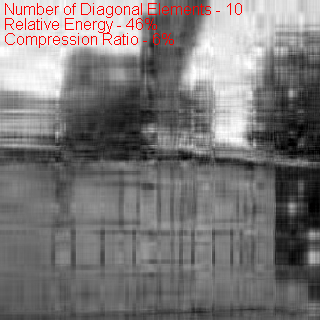
\includegraphics{Pullout10SingularValues.png}%
\end{minipage}
\\
\begin{minipage}[t]{0.3\columnwidth}%
\includegraphics{Pullout100SingularValues.png}%
\end{minipage}%
\begin{minipage}[t]{0.3\columnwidth}%
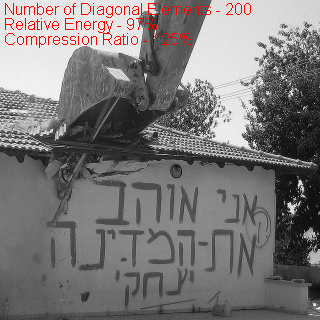
\includegraphics{Pullout200SingularValues.png}%
\end{minipage}
\begin{minipage}[t]{0.3\columnwidth}%
\includegraphics{Pullout240SingularValues.png}%
\end{minipage}

\end{itemize}

\lyxframeend{}\lyxframe{}

Applications of Order Reduction:
\begin{itemize}
\item Noise Reduction \\
Basic assumption - Noise is mainly pronounced in the small singular values. \\

\begin{minipage}[t]{0.22\columnwidth}
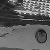
\includegraphics{NoiselessMatrix.png} \\
\tiny Noiseless Matrix
\end{minipage}%
\begin{minipage}[t]{0.22\columnwidth}
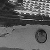
\includegraphics{NoisyMatrixStd1.png} \\
\tiny Noisy Matrix - Std 1
\end{minipage}
\begin{minipage}[t]{0.22\columnwidth}
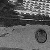
\includegraphics{NoisyMatrixStd6.png} \\
\tiny Noisy Matrix - Std 6
\end{minipage}
\begin{minipage}[t]{0.22\columnwidth}
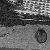
\includegraphics{NoisyMatrixStd11.png} \\
\tiny Noisy Matrix - Std 11
\end{minipage}


\end{itemize}

\lyxframeend{}\lyxframe{}
Analyzing the effect of noise on the Singular Values \\

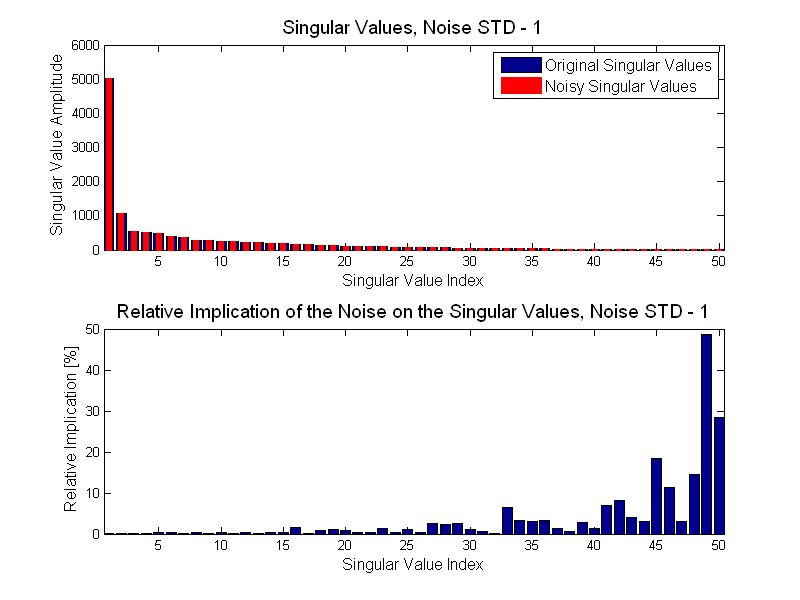
\includegraphics{NoiseReduction001Std1.png} \\

\lyxframeend{}\lyxframe{}
Analyzing the effect of noise on the Singular Values \\

\includegraphics{NoiseReduction002Std6.png} \\

\lyxframeend{}\lyxframe{}
Analyzing the effect of noise on the Singular Values \\

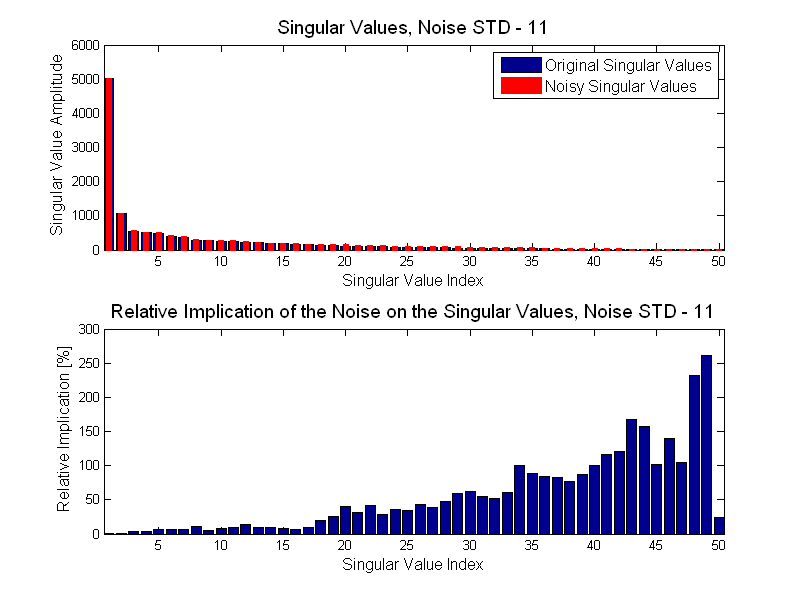
\includegraphics{NoiseReduction003Std11.png} \\


\lyxframeend{}\lyxframe{}
\begin{minipage}[t]{0.3\columnwidth}
\includegraphics{PulloutBW.png} \\
\tiny Ground Truth
\end{minipage}
\begin{minipage}[t]{0.3\columnwidth}

\includegraphics{NoisyPulloutStd6.png} \\
\tiny Added Noise Std 6
\end{minipage}
\begin{minipage}[t]{0.3\columnwidth}
\includegraphics{NoiseReducedPulloutStd6.png} \\
\tiny Reconstruction using 140 Singular Values
\end{minipage}


\lyxframeend{}\subsection{Solving Linear Equation System}

\lyxframeend{}\lyxframe{}
Consider the solution of the equation $ A x = b $.
\begin{itemize}
\item If $ b \in \mathcal{R} \left( A \right) $ there is at least one solution:
\begin{itemize}
\item If $ dim \left( \mathcal{N} \left( A \right) \right) = 0 $ there is only one unique solution, $ {x}_{r} \in \mathcal{R} \left( {A}^{H} \right) $, s.t. $ A {x}_{r} = b $.
\item If $ dim \left( \mathcal{N} \left( A \right) \right) \geq 1 $ , The columns of $ A $ are not independent, there are infinite solutions. Any vector of the form $ \hat{x} = {x}_{r} + {x}_{n} $ where $ {x}_{r} \in \mathcal{R} \left( {A}^{H} \right) $ is the solution from the previous case and $ {x}_{n} \in \mathcal{N} \left( A \right) $ is a solution s.t. $ A \left( {x}_{r} + {x}_{n} \right) = b $. \\
Which solution should be chosen? \\
Usually the solution with the minimum norm, $ {x}_{r} $.
\end{itemize}
\item If $ b \notin \mathcal{R} \left( A \right) $ there is no solution. \\
Usually, the following vector is searched, $ \hat{x} $ s.t. $ {\left\Vert A \hat{x} - b \right\Vert}_{2} $ is brought to minimum.
\end{itemize}


\lyxframeend{}\lyxframe{}
Assuming $ \hat{x} = \underset{x}{min} {\left\Vert A x - b \right\Vert}_{2} $. \\
By definition $ \hat{b} = A \hat{x} \in \mathcal{R} \left( A \right) $. \\
Meaning, the search is for $ \hat{b} $ s.t. $ {\left\Vert \hat{b} - b \right\Vert}_{2} $ is minimized.
\begin{center}
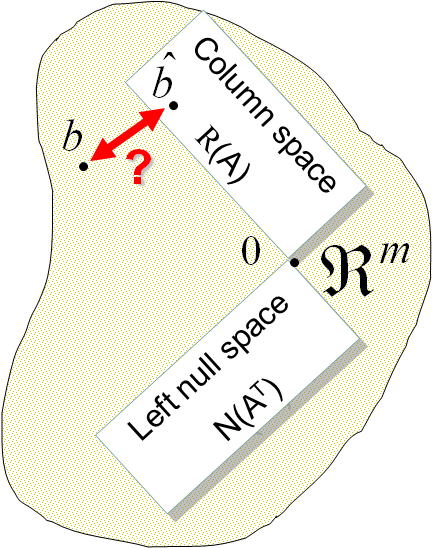
\includegraphics[scale = 0.25]{ErrorVector.PNG} \\
\end{center}


\lyxframeend{}\lyxframe{}
According to the Projection Theorem, only one vector $ \hat{b} $ exists s.t. $ {\left\Vert \hat{b} - b \right\Vert}_{2} $ is minimized. This vector is the projection of $ b $ on $ \mathcal{R} \left( A \right) $. \\
$$ \hat{b} = {Proj}_{\mathcal{R} \left( A \right)} \left( b \right) = {A}^{H} b $$
Moreover, 
$$ \hat{x} = \underset{x}{min} {\left\Vert A x - b \right\Vert}_{2} \Leftrightarrow \left( {A}^{H} A \right) \hat{x} = {A}^{H} b $$
Intuitively, the procedure is as following:
\begin{itemize}
\item Project $ b $ onto the Column Space $ \mathcal{R} \left( A \right) $, namely, $ \hat{b} = {Proj}_{\mathcal{R} \left( A \right)} \left( b \right) = {A}^{H} b $.
\item Project $ \hat{x} $ onto the Row Space $ \mathcal{R} \left( {A}^{H} \right) $, namely, $ {Proj}_{\mathcal{R} \left( {A}^{H} \right)} \left( \hat{x} \right) = A x $.
\item Project the previous result $ A x $ onto the Column Space $ \mathcal{R} \left( A \right) $, namely, $ {Proj}_{\mathcal{R} \left( A \right)} \left( A \hat{x} \right) = {A}^{H} \left( A \hat{x} \right) $.
\end{itemize}


\lyxframeend{}\lyxframe{}
The equation $ \left( {A}^{H} A \right) \hat{x} = {A}^{H} b $ is called the Normal Equations. If the columns of $ A $ are independent then $ {A}^{H} A $ is invertible and $ \hat{x} $ could be calculated as the following:
$$ \hat{x} = {\left( {A}^{H} A \right)}^{-1} {A}^{H} b $$
This is the Least Squares solution using the Pseudo Inverse of $ A $:
$$ {A}^{\dagger} = {\left( {A}^{H} A \right)}^{-1} {A}^{H} $$
\begin{center}
\includegraphics[scale = 0.20]{PseudoInverse.PNG}
\end{center}


\lyxframeend{}\lyxframe{}
Yet, if the columns of $ A $ are linearly dependent the Pseudo Inverse of $ A $ can't be calculated directly. \\
If $ A $ has dependent columns, then the null space of $ A $ is not trivial and there is no unique solution. \\
The problem becomes selecting one solution out of the infinite number of possible solutions. \\
As mentioned, commonly accepted approach is to select the solution with the smallest norm (Length). \\
This problem could be solved using the SVD and definition of the generalized Pseudo Inverse of a matrix.


\lyxframeend{}\lyxframe{}
\begin{block}{Definition}
The Pseudo Inverse of a matrix $ A = U \Sigma {V}^{H} $, denoted $ {A}^{\dagger} $ is given by
$$ {A}^{\dagger} = V {\Sigma}^{\dagger} {U}^{H} $$
Where $ {\Sigma}^{\dagger} $ is obtained by transposing $ \Sigma $ and inverting all non zero entries.
\end{block}

\begin{block}{Proposition III}
Let $ A = U \Sigma {V}^{H} $ and $ {x}^{\dagger} = {A}^{\dagger} b = V {\Sigma}^{\dagger} {U}^{H} b $. Then $ {A}^{H} A {x}^{\dagger} = {A}^{H} b $.
\end{block}

Namely, using the solution given by the Pseudo Inverse matrix calculated using the SVD holds the Normal Equations.
\textbf{This definition of Pseudo Inverse exists for any matrix}.


\lyxframeend{}\lyxframe{}
\begin{block}{Proposition III}
Let $ A = U \Sigma {V}^{H} $ and $ {x}^{\dagger} = {A}^{\dagger} b = V {\Sigma}^{\dagger} {U}^{H} b $. Then $ {A}^{H} A {x}^{\dagger} = {A}^{H} b $.
\end{block}

\begin{block}{proof}
It's sufficient to show that $ {A}^{H} \left( A {x}^{\dagger}- b \right) = 0 $.
\begin{eqnarray}
A {x}^{\dagger} - b & = & \left( U \Sigma {V}^{H} \right) V {\Sigma}^{\dagger} {U}^{H} b - b \nonumber \\
& = & \left(U \Sigma {\Sigma}^{\dagger} {U}^{H} - I \right) b \nonumber \\
& = & \left( U \left( \Sigma {\Sigma}^{\dagger} - I \right) {U}^{H} \right) b \nonumber
\end{eqnarray}
\end{block}


\lyxframeend{}\lyxframe{}
\begin{proof}[Proof. Continued]
Thus,
\begin{eqnarray}
{A}^{H} \left( A {x}^{\dagger} - b \right) & = & V {\Sigma}^{H} {U}^{H} U \left( \Sigma {\Sigma}^{\dagger} - I \right) {U}^{H} b \nonumber \\
& = & V {\Sigma}^{H} \left( \Sigma {\Sigma}^{\dagger} - I \right) {U}^{H} b \nonumber
\end{eqnarray}
One should observe that
$$ {\Sigma}^{H} = \begin{bmatrix} {\Sigma}^{H}_{r x r} & {0}_{r x \left( m - r \right)} \\
{0}_{\left( n - r \right) x r } & {0}_{\left( m - r \right) x \left( m - r \right)}
\end{bmatrix} $$
Where $ {\Sigma}_{r} $ is $ r $ by $ r $ submatrix of non zero diagonal entries in $ \Sigma $ and
$$ \Sigma {\Sigma}^{\dagger} - I  = \begin{bmatrix} {0}_{r x r} & {0}_{r x \left( m - r \right)} \\
{0}_{\left( n - r \right) x r } & {-I}_{\left( m - r \right) x \left( m - r \right)}
\end{bmatrix} $$
Hence the multiplication yields the zero matrix.
\end{proof}


\lyxframeend{}\lyxframe{}
\begin{block}{Proposition IV}
The vector $ \hat{x} = {A}^{\dagger} b $ is the shortest Least Squares solution to $ A x = b $, namely,
$$ {\left\Vert \hat{x} \right\Vert}_{2} = min \left\lbrace {\left\Vert x \right\Vert}_{2} : {\left\Vert A x - b \right\Vert}_{2} \ is \ minimal \right\rbrace $$
\end{block}

\begin{block}{proof}
Using the fact both $ U $ and $ V $ are Unitary
\begin{eqnarray}
\underset{{\left\Vert x \right\Vert}_{2}}{min} \left\lbrace \underset{x}{min} {\left\Vert A x - b \right\Vert}_{2} \right\rbrace & = & \underset{{\left\Vert x \right\Vert}_{2}}{min} \left\lbrace \underset{x}{min} {\left\Vert U \Sigma {V}^{H} x - b \right\Vert}_{2} \right\rbrace \nonumber \\
& = & \underset{{\left\Vert {V}^{H} x \right\Vert}_{2}}{min} \left\lbrace \underset{x}{min} {\left\Vert \Sigma {V}^{H} x - {U}^{H} b \right\Vert}_{2} \right\rbrace \nonumber \\
& = & \underset{{\left\Vert y \right\Vert}_{2}}{min} \left\lbrace \underset{x}{min} {\left\Vert \Sigma y - {U}^{H} b \right\Vert}_{2} \right\rbrace \nonumber
\end{eqnarray}
\end{block}


\lyxframeend{}\lyxframe{}
\begin{proof}
Observing at $ \underset{{\left\Vert y \right\Vert}_{2}}{min} \left\lbrace \underset{x}{min} {\left\Vert \Sigma y - {U}^{H} b \right\Vert}_{2} \right\rbrace $.
Since $ \Sigma $ is diagonal (Main diagonal to the least) there's only one Least Squares solution, $ \hat{y} = {\Sigma}^{\dagger} {U}^{H} b $.\\
Thus, 
$$ \hat{x} = V \hat{y} = V {\Sigma}^{\dagger} {U}^{H} b $$
will attain the minimum norm.
\end{proof}


\lyxframeend{}\lyxframe{}
As written previously, any solution which holds the Normal Equations is the Least Squares solution.
$$ \hat{x} = \underset{x}{min} {\left\Vert A x - b \right\Vert}_{2} \Leftrightarrow \left( {A}^{H} A \right) \hat{x} = {A}^{H} b $$
Yet, one should observe $ \hat{x} \in \mathcal{R} \left( {A}^{H} \right) $, namely, the solution lies in the Row Space of $ A $.
Hence, its norm is minimal among all solutions.
In short, the Pseudo Inverse simultaneously minimizes the norm of the error as well as the norm of the solution.


\lyxframeend{}\lyxframe{}
\begin{Large}
Example I
\end{Large} \\

Examining the following Linear System:
$$ A x = b $$
Where,
$$ A = \begin{bmatrix} 8 & 10 & 3 & 30 \\
9 & 6 & 6 & 18 \\
1 & 1 & 10 & 3
\end{bmatrix} , \ 
x = \begin{bmatrix} {x}_{1} \\
{x}_{2} \\
{x}_{3} \\
{x}_{4}
\end{bmatrix} = \begin{bmatrix} 1 \\
2 \\
3 \\
6
\end{bmatrix} , \
b = \begin{bmatrix} 217 \\
147 \\
51
\end{bmatrix} $$
Obviously, $ {A}^{-1} $ can't be calculated. Moreover, since $ rank \left( A \right) = 3 $ neither $ {\left({A}^{H} A \right)}^{-1} $ exists.
Yet the Pseudo Inverse using the SVD does exists.


\lyxframeend{}\lyxframe{}
Using the SVD approach $ A = U \Sigma {V}^{H} $. \\
Hence, $ {A}^{\dagger} = V {\Sigma}^{\dagger} {U}^{H} $. \\
Using MATLAB to calculate the SVD yields:
$$ \Sigma = \begin{bmatrix} 39.378 & 0 & 0 & 0 \\
0 & 10.002 & 0 & 0 \\
0 & 0 & 3.203 & 0
\end{bmatrix} 
\rightarrow
{\Sigma}^{\dagger} = \begin{bmatrix} 0.025 & 0 & 0 \\
0 & 0.1 & 0 \\
0 & 0 & 0.312 \\
0 & 0 & 0
\end{bmatrix} $$

Calculating $ \hat{x} $ yields:
$$ \hat{x} = V {\Sigma}^{\dagger} {U}^{H} b = \begin{bmatrix} 1 \\
2 \\
3 \\
6
\end{bmatrix} = x $$
The SVD canceled the 4th column which is dependent on the 2nd column of $ A $. \\
Since $ b \in \mathcal{R} \left( A \right) $ the exact solution could be calculated.


\lyxframeend{}\lyxframe{}
\begin{Large}
Example II
\end{Large} \\

In this case
$$ A = \begin{bmatrix} 5 & 0 & 0 & 0 \\
0 & 2 & 0 & 0 \\
0 & 0 & 0 & 0
\end{bmatrix} , \ 
x = \begin{bmatrix} {x}_{1} \\
{x}_{2} \\
{x}_{3} \\
{x}_{4}
\end{bmatrix} = \begin{bmatrix} 1 \\
2 \\
3 \\
6
\end{bmatrix} , \
b = \begin{bmatrix} 5 \\
4 \\
3
\end{bmatrix} $$
Obviously, $ b \notin \mathcal{R} \left( A \right) $.
Neither $ {A}^{-1} $ nor $ {\left( {A}^{H} A \right)}^{-1} $ exist.
Using the SVD Pseudo Inverse:
$$ \hat{x} = V {\Sigma}^{\dagger} {U}^{H} b = \begin{bmatrix} 1 \\
2 \\
0 \\
0
\end{bmatrix} $$

\lyxframeend{}\lyxframe{}
Examining the solution using the SVD. First, Since $ rank \left( A \right) = 2 $ its Column Space is spanned by the first 2 columns of $ U $. Calculating the projection of $ b $ onto the Column Space of $ A $ is given by $ \hat{b} = {Proj}_{\mathcal{R} \left( A \right)} \left( b \right) = \underset{i = 1}{\overset{2}{\sum}}{{U}^{i}}^{H} b {U}^{i} = \begin{bmatrix} 5 \\
4 \\
0
\end{bmatrix} $. \\
Now given the updated Linear System $ A \hat{x} = \hat{b} $ which has infinite number of solutions. \\
One could calculate that $ \mathcal{N} \left( A \right) = span \left( \begin{bmatrix} 0 \\
0 \\
1 \\
0
\end{bmatrix} , \begin{bmatrix} 0 \\
0 \\
0 \\
1
\end{bmatrix} \right) $. \\
Hence $ \hat{x} = \begin{bmatrix} \frac{{\hat{b}}_{1}}{{A}_{1, 1}} \\
\frac{{\hat{b}}_{2}}{{A}_{2, 2}} \\
0 \\
0
\end{bmatrix} + \left( s \begin{bmatrix} 0 \\
0 \\
1 \\
0
\end{bmatrix} + t \begin{bmatrix} 0 \\
0 \\
0 \\
1
\end{bmatrix} \right) = {\hat{x}}_{r} + {\hat{x}}_{n} $ where $ s, t \in \mathbb{R} $.


\lyxframeend{}\lyxframe{}
The target is the solution with the minimum norm. \\
Since $ {\hat{x}}_{r} \bot {\hat{x}}_{n} $ the norm of this solution is
$$ {\left\Vert \hat{x} \right\Vert}^{2} = {\left\Vert {\hat{x}}_{r} \right\Vert}^{2} + {\left\Vert {\hat{x}}_{n} \right\Vert}^{2} $$
The minimum norm solution is obtained by taking $ {x}_{n} = 0 $.\\
This results in the Pseudo Inverse solution as above.


\lyxframeend{}\lyxframe{}
\begin{Large}
Numerically Sensitive Problems
\end{Large} \\
Systems of equations that are poorly conditioned are sensitive to small change in values. \\
Since, practically speaking, there are always inaccuracies in measured data, the solution to these equations may be almost meaningless. \\
The SVD can help with the solution of ill-conditioned equations by identifying the direction of sensitivity and discarding that portion of the problem.
The procedure will be illustrated by the following example.


\lyxframeend{}\lyxframe{}
\begin{Large}
Example III
\end{Large} \\
Examining the following system of equations $ A x = b $
$$ \begin{bmatrix} 1 + 3 \epsilon & 1 - 3 \epsilon \\
3 - \epsilon & 3 + \epsilon \\
\end{bmatrix} \begin{bmatrix} {x}_{1} \\
{x}_{2}
\end{bmatrix} = \begin{bmatrix} {b}_{1} \\
{b}_{2}
\end{bmatrix} $$
The SVD of $ A $ is
$$ A = \frac{1}{\sqrt{20}} \begin{bmatrix} 1 & 3 \\
3 & -1
\end{bmatrix} \begin{bmatrix} 2 \sqrt{5} &  \\
 & 2 \epsilon \sqrt{5}
\end{bmatrix} \begin{bmatrix} 1 & 1 \\
1 & -1
\end{bmatrix} $$
From which the exact inverse of $ A $ is
$$ {A}^{-1} = \sqrt{20} \begin{bmatrix} 1 & 1 \\
1 & -1
\end{bmatrix} \begin{bmatrix} \frac{1}{2 \sqrt{5}} &  \\
 & \frac{1}{2 \epsilon \sqrt{5}}
\end{bmatrix} \begin{bmatrix} 1 & 3 \\
3 & -1
\end{bmatrix} = \frac{1}{20} \begin{bmatrix} 1 + \frac{3}{\epsilon} & 3 - \frac{1}{\epsilon} \\
1 - \frac{3}{\epsilon} & 3 + \frac{1}{\epsilon}
\end{bmatrix} $$
Easily, one can convince himself that for small $ \epsilon $ the matrix $ {A}^{-1} $ has large entries which makes $ x = {A}^{-1} b $ unstable.


\lyxframeend{}\lyxframe{}
Observe that the entry $ \frac{1}{2 \epsilon \sqrt{5}} $ multiplies the column $ \begin{bmatrix}
1 \\
-1
\end{bmatrix} $. This is the sensitive direction. As $ b $ changes slightly, the solution changes in a direction mostly along the sensitive direction. \\
If $ \epsilon $ is small, $ {\sigma}_{2} = 2 \epsilon \sqrt{5} $ may be set to zero to approximate $ A $.
$$ A \approx \frac{1}{\sqrt{20}} \begin{bmatrix} 1 & 3 \\
3 & -1
\end{bmatrix} \begin{bmatrix} 2 \sqrt{5} &  \\
 & 0
\end{bmatrix} \begin{bmatrix} 1 & 1 \\
1 & -1
\end{bmatrix} $$
The Pseudo Inverse is
$$ {A}^{\dagger} = \sqrt{20} \begin{bmatrix} 1 & 1 \\
1 & -1
\end{bmatrix} \begin{bmatrix} \frac{1}{2 \sqrt{5}} &  \\
 & 0
\end{bmatrix} \begin{bmatrix} 1 & 3 \\
3 & -1
\end{bmatrix} = \frac{1}{20} \begin{bmatrix} 1 & 3 \\
1 & 3
\end{bmatrix} $$
In this case the multiplier of the sensitive direction vector is zero, no motion in the sensitive direction occurs. Any Least Squares solution to the equation $ A x = b $ is of the form $ \hat{x} = {A}^{\dagger} b $ so that $ \hat{x} = c \begin{bmatrix}
1 \\
1
\end{bmatrix} $ for $ c \in \mathbb{R} $, meaning perpendicular to the sensitive direction.


\lyxframeend{}\lyxframe{}
As this example illustrates, the SVD identifies the stable and unstable directions of the problem and, by zeroing small singular values, eliminates the unstable directions. \\
The SVD could be used to both illustrate poor conditioning and provide a cure for the ailment. For the equation $ A x = b $ with solution $ x = {A}^{-1} b $, writing the solution using the SVD:
$$ x = {A}^{-1}b = {\left(U \Sigma {V}^{H} \right)}^{-1} = \underset{i = 1}{\overset{r}{\sum}} {v}_{i} \frac{{u}_{i}^{H}b}{{\sigma}_{i}} $$
If the singular value $ {\sigma}_{i} $ is small, then a small change in $ b $ or a small change in either $ U $ or $ V $ may be amplified into a large change in the solution $ x $. A small singular value responds to a matrix which is nearly singular and thus more difficult to invert accurately.


\lyxframeend{}\lyxframe{}
Another point of view, considering the equation
$$ A {x}_{0} = {b}_{0} \Rightarrow {x}_{0} = {A}^{-1} {b}_{0} $$
Let $ b = {b}_{0} + \delta b $ where $ \delta b $ is the error or noise, etc. \\
Therefore
$$ A x = {b}_{0} + \delta b \Rightarrow x = {A}^{-1} {b}_{0} + {A}^{-1} \delta b = {x}_{0} + \delta x $$
Investigating how small or large is this error in the answer for a given amount of error. Note that
$$ \delta x = {A}^{-1} \delta b \Rightarrow \left\Vert \delta x \right\Vert \leq \left\Vert {A}^{-1} \right\Vert \left\Vert \delta b \right\Vert $$
Or since $ \left\Vert {A}^{-1} \right\Vert  = {\sigma}_{max} \left( {A}^{-1} \right) = \frac{1}{{\sigma}_{min} \left( A \right)} $ the following holds
$$ \left\Vert \delta x \right\Vert \leq \frac{\left\Vert \delta b \right\Vert}{{\sigma}_{min} \left( A \right)} $$


\lyxframeend{}\lyxframe{}
However recalling that $ {x}_{0} = {A}^{-1} {b}_{0} $ and therefore
$$ \left\Vert {x}_{0} \right\Vert \geq {\sigma}_{min} \left( {A}^{-1} \right) \left\Vert {b}_{0} \right\Vert = \frac{\left\Vert {b}_{0} \right\Vert}{{\sigma}_{max} \left( A \right)} $$
Combining the equations yields
$$ \frac{\left\Vert \delta x \right\Vert}{\left\Vert {x}_{0} \right\Vert} \leq \frac{\left\Vert \delta b \right\Vert}{\left\Vert {b}_{0} \right\Vert} \frac{{\sigma}_{max} \left( A \right)}{{\sigma}_{min} \left( A \right)} $$
The last fraction, $ \frac{{\sigma}_{max} \left( A \right)}{{\sigma}_{min} \left( A \right)} $, is called 'The Condition Number of $ A $'.\\
This number is indicative of the magnification of error in linear equation of interest. In most problems, a matrix with very large condition number is called ill conditioned and will result in severe numerical difficulties.


\lyxframeend{}\lyxframe{}
The solution to those numerical difficulties using the SVD is basically rank reduction:
\begin{enumerate}
\item Compute the SVD of $ A $.
\item Examine the singular values of $ A $ and zero out any that are "small" to obtain a new approximate $ \Sigma $ matrix.
\item Compute the solution by $ \hat{x} = V {\Sigma}^{\dagger} {U}^{H} b $.
\end{enumerate}
Determining which singular values are "small" is problem dependent and requires some judgment. \\


\lyxframeend{}\subsection{Total Least Squares}


\lyxframeend{}\lyxframe{}
In the classic Least Squares problems, the solution minimizing $ {\left\Vert A x - b \right\Vert}_{2} $ is sought after. The hidden assumption is that matrix $ A $ is correct, any error in the problem is in $ b $. \\
The Least Squares problem finds a vector $ \hat{x} $ s.t.
$$ {\left\Vert A \hat{x} - b \right\Vert}_{2} = min $$
which is accomplished by finding some perturbation $ r $ of the right hand side of minimum norm
$$ A x = b + r $$ 
s.t. $ \left( b + r \right) \in \mathcal{R} \left( A \right) $.
In the Total Least Squares problem, both the right and left side of the equation assumed to have errors. The solution of the perturbed equation
$$ \left( A + E \right) x = b + r $$
is sought s.t. $ \left( b + r \right) \in \mathcal{R} \left( A + E \right) $ and the norm of the perturbations is minimized.


\lyxframeend{}\lyxframe{}
Intuitively, The right hand side is "bent" toward the left hand side while the left hand side is "bent" toward the right hand side. \\
\includegraphics[scale = 0.30]{LS01.PNG}
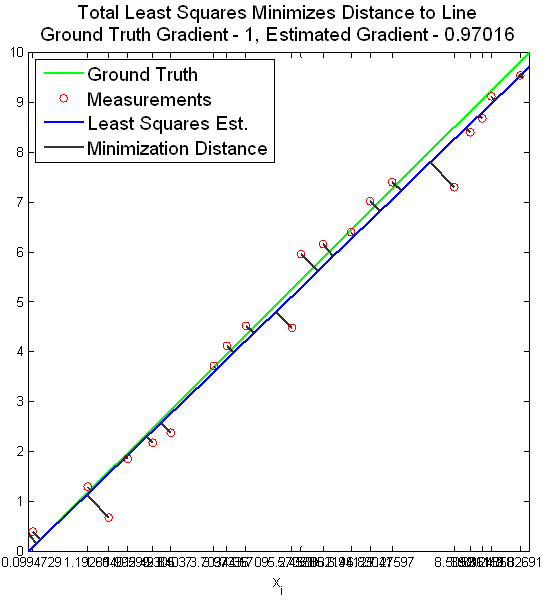
\includegraphics[scale = 0.30]{TLS01.PNG}

\lyxframeend{}\lyxframe{}
Let $ A $ be an $ m x n $ matrix. To find the solution to the TLS problem one may observe the homogeneous form
$$ \begin{bmatrix}
A + E | b + r
\end{bmatrix}
\begin{bmatrix}
x \\
-1
\end{bmatrix} = 0 \rightarrow 
\left(\begin{bmatrix}
A | b
\end{bmatrix} + 
\begin{bmatrix}
E | r
\end{bmatrix} \right)
\begin{bmatrix}
x \\
-1
\end{bmatrix} = 0 $$
Let $ C = \begin{bmatrix}
A | b
\end{bmatrix} \in {\mathbb{C}}^{m x \left( n + 1 \right)} $ and let $ \Delta = \begin{bmatrix}
E | r
\end{bmatrix} $ be the perturbation of the data. In order for the homogeneous form to have solution the vector $ \begin{bmatrix}
{x} \\
-1
\end{bmatrix} $ must lie in the Null Space of $ C + \Delta $ and in order for the solution not to be trivial, the perturbation $ \Delta $ must be such that $ C + \Delta $ is rank deficient.


\lyxframeend{}\lyxframe{}
Analyzing the TLS problem using the SVD.
We bring $ \left(A + E \right) x = \left( b + r \right) $ into the form 
$$ \begin{bmatrix}
A + E | b + r
\end{bmatrix}
\begin{bmatrix}
x \\
-1
\end{bmatrix} = 0 $$
Let $ \begin{bmatrix}
A + E | b + r
\end{bmatrix} = U \Sigma {V}^{H} $ be the SVD of the above form.
If $ {\sigma}_{n + 1} \neq 0 $ then $ rank \left( \begin{bmatrix}
A + E | b + r
\end{bmatrix} \right) = n + 1 $ which means the $ \mathcal{R} \left( \begin{bmatrix}
A + E | b + r
\end{bmatrix} \right) = {\mathbb{R}}^{n + 1} $, hence there's no nonzero vector in the orthogonal complement of the Row Space hence the set of equations is incompatible. To obtain solution the rank of $ \begin{bmatrix}
A + E | b + r
\end{bmatrix} $ must be reduced to $ n $. \\
As shown before the best approximation of rank $ n $ in both Frobenius and $ {l}_{2} $ norm is given by the SVD
$$ \begin{bmatrix}
\hat{A} | \hat{b}
\end{bmatrix} = U \hat{\Sigma} {V}^{H}, \quad \hat{\Sigma} = diag \left( {\sigma}_{1}, {\sigma}_{2}, \ldots , {\sigma}_{n}, 0 \right) $$


\lyxframeend{}\lyxframe{}
The minimal TLS correction is given by
$$ {\sigma}_{n + 1} = \underset{rank \left( \begin{bmatrix}
\hat{A} | \hat{b}
\end{bmatrix} \right) = n}{min} {\left\Vert \begin{bmatrix}
A | b
\end{bmatrix} - \begin{bmatrix}
\hat{A} | \hat{b}
\end{bmatrix} \right\Vert}_{F} $$
Attained for
$$ \begin{bmatrix}
E | r
\end{bmatrix} = {\sigma}_{n + 1} {u}_{n + 1} {v}_{n + 1}^{H} $$
Note that the TLS correction matrix has rank one. \\
It is clear that the approximate set $ \begin{bmatrix}
\hat{A} | \hat{b}
\end{bmatrix} \begin{bmatrix}
x \\
-1
\end{bmatrix} = 0 $ is compatible and the solution is given by the only vector, $ {v}_{n + 1} $, that belongs to $ \mathcal{N} \left( \begin{bmatrix}
\hat{A} | \hat{b}
\end{bmatrix} \right) $. \\
The TLS solution is obtained by scaling $ {v}_{n + 1} $ until its last component equals to $ -1 $, or
$$ \begin{bmatrix}
x \\
-1
\end{bmatrix} = \frac{-1}{{V}_{n + 1, n + 1}} {v}_{n + 1} $$


\lyxframeend{}\lyxframe{}
For simplicity it assumed that $ {V}_{n + 1, n + 1} \neq 0 $ and $ {\sigma}_{n} > {\sigma}_{n + 1} $ hence the solution exists and it is unique. Otherwise, the solution might not exists or isn't unique (Any superposition of few columns of $ V $).
For complete analysis of the existence and uniqueness of the solution see [].
\vskip0pt plus.5fill
Basic algorithm of the TLS would be:\\
Given $ A x \approx b $, where $ A \in {\mathbb{C}}^{m x n}, b \in {\mathbb{C}}^{m} $ the TLS solution could be obtained by
\begin{itemize}
\item Compute the SVD of $ \begin{bmatrix}
A | b
\end{bmatrix} = U \Sigma {V}^{H} $.
\item If $ {V}_{n + 1, n + 1} \neq 0 $ the TLS solution would be 
$$ {x}_{TLS} = \frac{-1}{{V}_{n + 1, n + 1}} {v}_{n + 1} \left( 1:n \right) $$
\end{itemize}


\lyxframeend{}\lyxframe{}
The geometric properties of the solution could be described as following, the TLS solution minimizes the distance between the vector $ b $ to the plane defined by the solution $ {x}_{TLS} $.

\vskip0pt plus.1fill

Let $ C = U \Sigma {V}^{H} $ From the definition of the $ {l}_{2} $ Norm of a matrix
$$ \frac{{\left\Vert C v \right\Vert}_{2}}{{\left\Vert v \right\Vert}_{2}} \geq {\sigma}_{n + 1} $$
Where $ {\left\Vert v \right\Vert}_{2} \neq 0 $. Equality holds if and only if $ v \in {S}_{c} $ where $ {S}_{c} = span \left\lbrace {v}_{i} \right\rbrace $ and $ {v}_{i} $ are the columns of $ V $ which satisfy $ {u}_{i}^{H} C {v}_{i} = {\sigma}_{n + 1} $. \\
The TLS problem amounts to finding vector $ x $ s.t.
$$ \frac{{\left\Vert \begin{bmatrix}
A | b
\end{bmatrix} \begin{bmatrix}
x \\
-1
\end{bmatrix} \right\Vert}_{2}}{{\left\Vert \begin{bmatrix}
x \\
-1
\end{bmatrix} \right\Vert}_{2}} = {\sigma}_{n + 1} $$


\lyxframeend{}\lyxframe{}
By squaring everywhere
$$ \underset{x}{min} \frac{{\left\Vert \begin{bmatrix}
A | b
\end{bmatrix} \begin{bmatrix}
x \\
-1
\end{bmatrix} \right\Vert}_{2}^{2}}{{\left\Vert \begin{bmatrix}
x \\
-1
\end{bmatrix} \right\Vert}_{2}^{2}} = \underset{x}{min} \underset{i = 1}{\overset{m}{\sum}} \frac{{\left| {A}_{i}^{H} x - {b}_{i} \right|}^{2}}{{x}^{H} x + 1} $$

The quantity $ \frac{{\left| {A}_{i}^{H} x - {b}_{i} \right|}^{2}}{{x}^{H} x + 1} $ is the square of the distance from the point $ \begin{bmatrix}
{A}_{i}^{H} \\
b
\end{bmatrix} \in {\mathbb{C}}^{n + 1} $ to the nearest point on the hyperplane $ P $ defined by 
$$ P = \left\lbrace \begin{bmatrix}
a \\
b
\end{bmatrix} | a \in {\mathbb{C}}^{n}, b \in \mathbb{C}, b = {x}^{H} a \right\rbrace $$
So the TLS problem amounts to finding the closest hyperplane to the set of points $ \left\lbrace \begin{bmatrix}
{A}_{1}^{H} \\
{b}_{1}
\end{bmatrix} , \begin{bmatrix}
{A}_{2}^{H} \\
{b}_{2}
\end{bmatrix}, \ldots , \begin{bmatrix}
{A}_{m}^{H} \\
{b}_{m}
\end{bmatrix} \right\rbrace $.


\lyxframeend{}\lyxframe{}
The minimum distance property can be shown as following.
Let $ P $ be the plane orthogonal to the normal vector $ n \in {\mathbb{R}}^{n + 1} $ s.t.
$$ P = \left\lbrace r \in {\mathbb{C}}^{n + 1} : {r}^{H} n = 0 \right\rbrace $$
and let $ n $ have the following form $ n = \begin{bmatrix}
x \\
-1
\end{bmatrix} $. Let $ p = \begin{bmatrix}
{A}_{m}^{H} \\
{b}_{m}
\end{bmatrix} $ be a point in $ {\mathbb{C}}^{n + 1} $. Finding a point, $ q \in {\mathbb{C}}^{n + 1} $ which belongs to the plane $ P $ and is closest to the point $ p $ is a constrained optimization problem, minimize $ \left\Vert p - q \right\Vert $ subject to $ {n}^{H} q = 0 $. The minimization function
\begin{eqnarray}
J \left( q \right) & = & {\left\Vert p - q \right\Vert}^{2} + 2 \lambda {n}^{H} q = {p}^{H}p - 2 {p}^{H} q + 2 \lambda {n}^{H} q + {q}^{H} q \nonumber \\
& = & {\left( q - p + \lambda n \right)}^{2} \left( q - p + \lambda n \right) + 2 \lambda {p}^{H}n - {\lambda}^{2}{n}^{H}n \nonumber
\end{eqnarray}
This is clearly minimized when $ q = p - \lambda n $. 


\lyxframeend{}\lyxframe{}
Determining $ \lambda $ by the constrain
$$ {n}^{H} q = {n}^{H}p - \lambda {n}^{H} n = 0 \rightarrow \lambda = \frac{{n}^{H} p }{{n}^{H} n} $$
Inserting results into the "Minimization Function" yields
\begin{eqnarray}
J \left( q \right) & = & 2 \lambda {p}^{H} n - {\lambda}^{2} {n}^{H} n \nonumber \\
& = & \frac{2 {n}^{H} p p {p}^{H} n}{{n}^{H} n} - \frac{{n}^{H} n {p}^{H} p {n}^{H} n}{{n}^{H} n {n}^{H} n} \nonumber \\
& = & \frac{{\left( {n}^{H} p \right)}^{2}}{{n}^{H} n} = \frac{{\left( {x}^{H} {A}_{m} - {b}_{m} \right)}^{2}}{{x}^{H} x + 1} \nonumber
\end{eqnarray}
Alternative solution using the "Projection Theorem". The distance from the point $ p $ to the plane $ P $ can be found by finding the length of the projection of $ p $ onto $ n $, which yields
$$ {d}_{min}^{2} \left( p, P \right) = \frac{{\left\langle p, n \right\rangle}^{2}}{{\left\Vert n \right\Vert}^{2}} = \frac{\begin{bmatrix}
{x}^{H}, -1
\end{bmatrix} \begin{bmatrix}
{{A}_{m}}^{H} \\
{b}_{m}
\end{bmatrix}}{{x}^{H} x + 1} $$ 


\lyxframeend{}\subsection{Principal Component Analysis}
\lyxframeend{}\lyxframe{}
Principal Component Analysis (PCA) is the mathematical procedure that uses an orthogonal transformation to convert a set of observations of possibly correlated variables into a set of values of uncorrelated variables called Principal Components. \\
The number of Principal Components is less than or equal to the number of original variables. \\
This transformation is defined in such way that the first component has a variance as high as possible (That's, accounts for as much of the variability in data as possible), and each succeeding component in turn has the highest variance possible under the constraint that it is orthogonal to (Uncorrelated with) the preceding components.


\lyxframeend{}\lyxframe{}
PCA is mathematically defined as an orthogonal linear transformation that transforms the data to a new coordinate system such that the greatest variance by any projection of the data comes to lie on the first coordinate (Called the first Principal Component), the second greatest variance on the second coordinate and so on. \\
Assuming given a collection of data of columns vectors $ {a}_{1}, {a}_{2}, \ldots , {a}_{m} \in {\mathbb{R}}^{n} $. \\
The projection of the data onto a subspace $ U \in {\mathbb{R}}^{r}, r \leq m $ which is is spanned by the orthogonal basis $ {u}_{1}, {u}_{2}, \ldots, {u}_{r} $ is given by
$$ {a}_{i} = {f}_{i1} {u}_{1} + {f}_{i2} {u}_{2} + \ldots + {f}_{ir} {u}_{r}, i=1:m $$
for some coefficients $ {f}_{ij} $. \\
Note that $ {f}_{ij} = {a}_{i}^{H} {u}_{j} $, the projection of $ {a}_{i} $ along the direction of $ {u}_{j} $. \\
By the Projection Theorem This projection is the closest in the $ {l}_{2}-norm $ sense to the data given by $ {a}_{i} $.


\lyxframeend{}\lyxframe{}
The search is after the orthogonal basis $ {u}_{1}, {u}_{2}, \ldots, {u}_{r} $. \\
Formulation the constraint of maximization of the variance along the direction of $ {u}_{1} $ yields
$$ \underset{\left\Vert w \right\Vert = 1}{max} \underset{i = 1}{\overset{m}{\sum}} {\left| {a}_{i}^{H} w \right|}^{2} = {\left\Vert {A}^{H} w \right\Vert}^{2} = {\left({A}^{H} w \right)}^{H} \left( {A}^{H} w \right) = {w}^{H} A {A}^{H} w $$
Using the SVD of $ A = U \Sigma {V}^{H} $, Then $ A {A}^{H} = U \Sigma {\Sigma}^{H} {U}^{H} $. \\
Observing,
$$ \frac{{w}^{H} A {A}^{H} w}{{w}^{H} w} = \frac{{\left( {U}^{H} w \right)}^{H} \Sigma {\Sigma}^{H} \left( {U}^{H} w \right)}{{\left( {U}^{H} w \right)}^{H} \left( {U}^{H} w \right)} $$
Noticing that there are only $ r $ non zero entries in $ \Sigma $ by the properties the SVD. Defining $ x = {U}^{H} w $ yields
$$ \frac{{w}^{H} A {A}^{H} w}{{w}^{H} w} = \frac{{\sigma}_{1}^{2} {x}_{1}^{2} + {\sigma}_{2}^{2} {x}_{2}^{2} + \ldots + {\sigma}_{r}^{2} {x}_{r}^{2}}{{x}_{1}^{2} + {x}_{2}^{2} + \ldots + {x}_{m}^{2}} $$


\lyxframeend{}\lyxframe{}
Now we have
$$ \underset{w \neq 0}{max} \frac{{w}^{H} A {A}^{H} w}{{w}^{H} w} = \underset{w \neq 0}{max} \frac{{\sigma}_{1}^{2} {x}_{1}^{2} + {\sigma}_{2}^{2} {x}_{2}^{2} + \ldots + {\sigma}_{r}^{2} {x}_{r}^{2}}{{x}_{1}^{2} + {x}_{2}^{2} + \ldots + {x}_{m}^{2}} $$
Assuming $ {\sigma}_{1} \geq {\sigma}_{2} \geq \ldots \geq {\sigma}_{r} $. \\
Then 
$$ \underset{w \neq 0}{max} \frac{{\sigma}_{1}^{2} {x}_{1}^{2} + {\sigma}_{2}^{2} {x}_{2}^{2} + \ldots + {\sigma}_{r}^{2} {x}_{r}^{2}}{{x}_{1}^{2} + {x}_{2}^{2} + \ldots + {x}_{m}^{2}} = {\sigma}_{1}^{2} = {\lambda}_{1} $$
Which the largest eigenvalue of $ A $.
The vector $ x $ which makes the maximum is $ {x}_{1} = 1 $ and $ {x}_{i} = 0 $ for $ i = 2 : m $. Which corresponds to $ w = U x = {u}_{1} $. \\
The first Principal Component is indeed achieved by the first eigenvector $ {u}_{1} $ of $ A {A}^{H} $.


\lyxframeend{}\lyxframe{}
Calculating the second Principal Component under the constraint being orthogonal to the first and maximizing the projection
$$ \underset{\left\Vert w \right\Vert = 1, {w}^{H} {u}_{1} = 0}{max} \underset{i = 1}{\overset{m}{\sum}} {\left| {a}_{i}^{H} w \right|}^{2} = \underset{w \neq 0, {w}^{H} {u}_{1} = 0}{max} \frac{{w}^{H} \left( A {A}^{H} \right) w}{{w}^{H} w} $$
Using the definition from above yields
\begin{eqnarray}
\underset{x \neq 0, {x}^{H} {U}^{H} {u}_{1} = 0}{max} \frac{{\sigma}_{1}^{2} {x}_{1}^{2} + {\sigma}_{2}^{2} {x}_{2}^{2} + \ldots + {\sigma}_{r}^{2} {x}_{r}^{2}}{{x}_{1}^{2} + {x}_{2}^{2} + \ldots + {x}_{m}^{2}} = \nonumber \\
\underset{x \neq 0, {x}_{1} = 0}{max} \frac{{\sigma}_{1}^{2} {x}_{1}^{2} + {\sigma}_{2}^{2} {x}_{2}^{2} + \ldots + {\sigma}_{r}^{2} {x}_{r}^{2}}{{x}_{1}^{2} + {x}_{2}^{2} + \ldots + {x}_{m}^{2}} = {\sigma}_{2}^{2} = {\lambda}_{2} \nonumber
\end{eqnarray}
Which is the second largest eigenvalue of $ A {A}^{H} $. \\
The vector $ x $ which makes the maximum is $ {x}_{2} = 1 $ and $ {x}_{i} = 0 $ for $ i = 1, 3 : m $. \\
This corresponds to $ w = U x = {u}_{2} $, The second Eigenvector, $ {u}_{2} $, of $ A {A}^{H} $.


\lyxframeend{}\lyxframe{}
Continuing this pattern, $ {u}_{i} $ is the $ i $th Principal Component. \\
The set of orthogonal vectors which spans the subspace the data is projected to and maximizes the variance of the data is the first $ r $ vectors which consists the orthogonal matrix from the SVD, $ U $. \\
Observing the SVD yields the the result immediately
$$ A = U \Sigma {V}^{H} \rightarrow Y = {U}^{H} A = \Sigma {V}^{H} $$
Observing the scatter matrix of $ Y $
$$ {C}_{Y} = Y {Y}^{H} = {U}^{H} A {\left( {U}^{H} A \right)}^{H} = {U}^{H} A {A}^{H} U = {U}^{H} {C}_{X} U $$
Since the matrix $ U $ is the Eigenvectors matrix of $ {C}_{X} = X {X}^{H} $ by the Diagonalization Theorem $ {C}_{Y} $ is diagonal.
Another look yields
$$ Y {Y}^{H} = \Sigma {V}^{H} {\left( \Sigma {V}^{H} \right)}^{H} = \Sigma {V}^{H} V {\Sigma}^{H} = \Sigma {\Sigma}^{H} = diag({\sigma}_{1}^{2}, {\sigma}_{2}^{2}, \ldots, {\sigma}_{r}^{2}) $$
Namely, the Scatter matrix, hence the Covariance Matrix of $ Y $ is diagonal. Moreover, The constraint on the variance holds.


\lyxframeend{}\section*{Summary}


\lyxframeend{}\lyxframe{}
\begin{itemize}
\item The SVD is a decomposition \textcolor{red}{which can be applied on any matrix}.
\item The SVD \textcolor{red}{exposes fundamental properties} of a linear operator such as the fundamental spaces, Frobenius Norm and $ {l}_{2} $ Norm.
\item The SVD \textcolor{red}{can be utilized in many applications} such as solving linear systems (Least Squares, Total Least Squares) and order reduction (Compression, Noise Reduction, Principal Component Analysis).
\end{itemize}


\vskip0pt plus.5fill
\begin{itemize}
\item To Be Continued

\begin{itemize}
\item Regulating Linear Equations System.
\end{itemize}
\end{itemize}

\lyxframeend{}

\appendix

\lyxframeend{}\section*{Appendix}


\lyxframeend{}\subsection*{For Further Reading}


\lyxframeend{}\lyxframe{[allowframebreaks]}

\beamertemplatebookbibitems
\begin{thebibliography}{References}
\bibitem{Author1990}A. Author.\newblock\emph{Handbook of Everything}.\newblock
Some Press, 1990.\beamertemplatearticlebibitems

\bibitem{Someone2002}S. Someone.\newblock On this and that\emph{.}
\newblock\emph{Journal on This and That}. 2(1):50--100, 2000.

\bibitem{Royi01}R. Avital.\newblock On this and that\emph{.}
\newblock\emph{Journal on This and That}. 2(1):50--100, 2000.

\end{thebibliography}

\lyxframeend{}
\end{document}
